\chapter{Complex Prominence Emission Through\\2D Cylindrical Radiative Transfer Modelling}\label{Chap:2DModel}

Prominences are inherently 3D structures and must be treated as such. Here we explore the use of cylindrical geometry with radiative transfer calculated along a `single slit' focused on the centre of this geometry. We can also stack several different cylinders of varying thermodynamic parameters to produce complex line profiles akin to the line profiles that 1D modelling struggles, or even fails, to model. Here we make use of the 2D NLTE RT code, RTCY described in \sect{rtcyintro}.



\section{Effects of Velocity on Line Formation}
%\section{Single Thread Simulations}
As RTCY includes a variety of velocity settings, and we can investigate how these affect the line formation. Initially we investigate the formation of the lines in the static case, as presented in \fig{fig:exhmg}. We can investigate the line formation here by consulting the corresponding Carlsson and Stein plots.

\begin{figure}
    \centering
    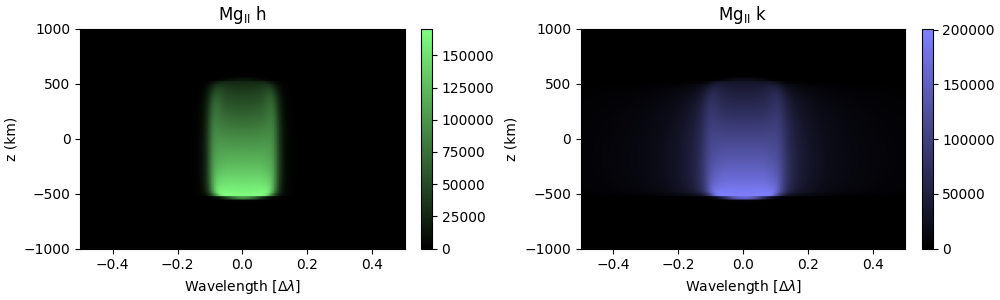
\includegraphics[width=\linewidth]{./03Modelling2D/figs/exmg.png}
    \caption[Output of RTCY for the h\&k lines of once-ionised magnesium.]{Output of RTCY for the h\&k lines of once-ionised magnesium. The units of the colourbars are \cgsint. The parameters of this example run are; $P=0.1$~dyn~cm$^{-2}$, $r_0=500$~km, $r_1=1000$~km, $T_0=6000$~K, $T_1=100~000$~K, $v_T=5$~km~s$^{-1}$, $\alpha=\frac{\pi}{2}$~rad and $H=10000$~km with no velocity setting active.}
    \label{fig:exhmg}
\end{figure}

\begin{figure}
    \centering
    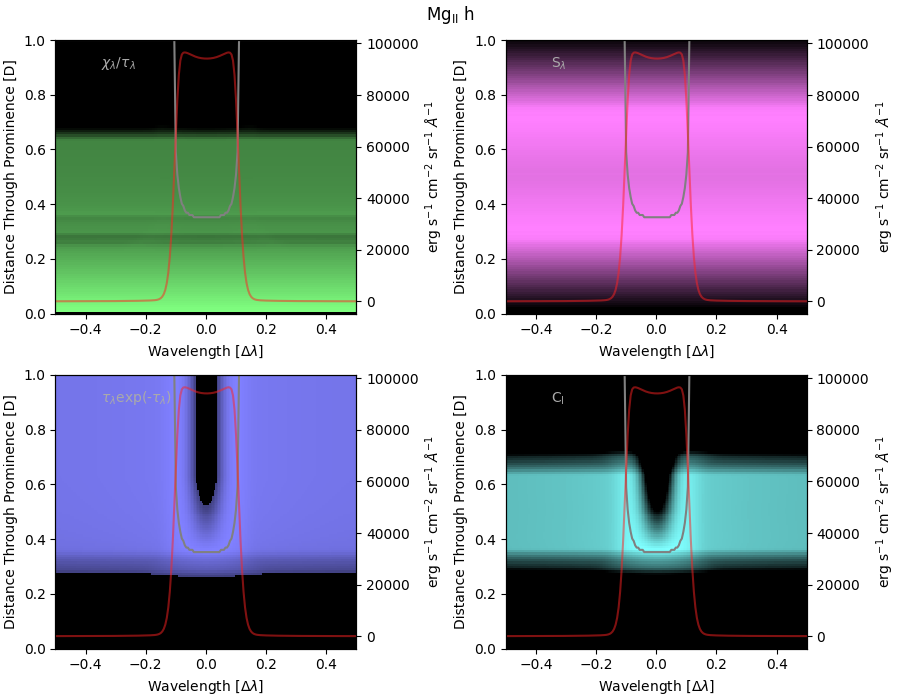
\includegraphics[width=0.9\linewidth]{./03Modelling2D/figs/matplots/mghv0.png}
    \caption[The various plots that break down the contribution function.]{The various plots that break down the contribution function for the line at $z=0$ for the run in \fig{fig:exhmg}. The $\tau=1$ line is drawn on each of these plots in light grey, and the line profile is drawn in red. The left y axis is the distance through the prominence and is defined from the POV of the LOS. So 0 is the front of the prominence and 1 is the back. The right y axis is for the line profile.}
    \label{v0}
\end{figure}
\fig{v0} shows us this plot for \mgii~h. \mgii~k is similar to \mgii~h, and will be omitted. These plots are taken from the centre of the hypothetical slit spectrograph ($z=0$). Distance through the prominence is measured along the line of sight with $D=0$ being the front of the prominence and $D=1$ being the back, as opposed to through the atmosphere as these plots are conventionally presented.
\begin{figure}
    \centering
    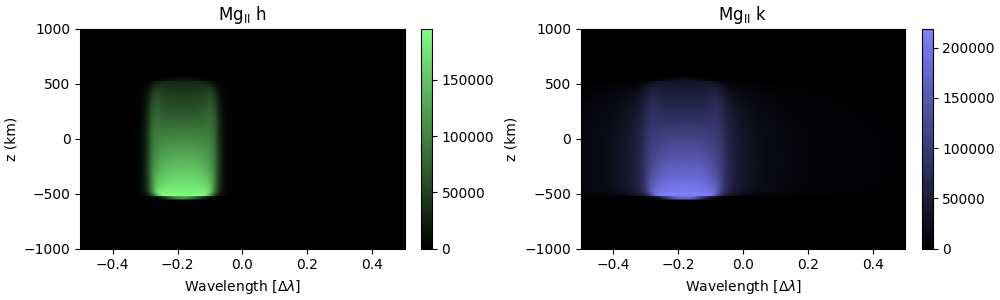
\includegraphics[width=\linewidth]{./03Modelling2D/figs/matplots/mgvy20cont.png}
    \caption{The \mgiihk{} lines formed when $v_y=20$\kms. We see a simple blueshift. The remaining parameters are the same as \fig{fig:exhmg}.}
    \label{v20} \vspace{20pt}
    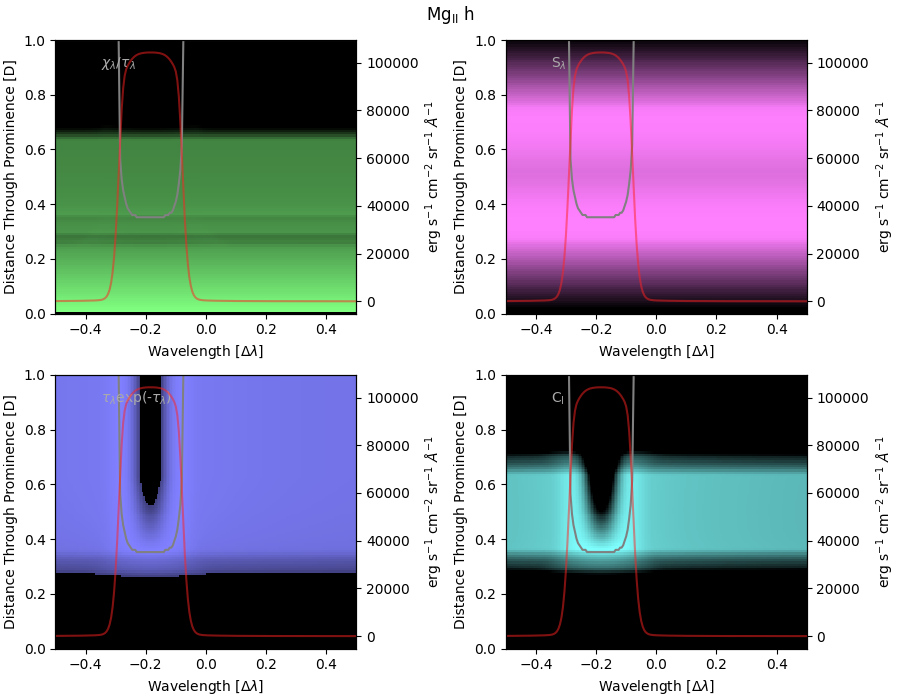
\includegraphics[width=\linewidth]{./03Modelling2D/figs/matplots/mghvy20.png}
    \caption{Same as \fig{v0} but for \fig{v20}.}
    \label{vh20}
\end{figure}
\newpage
$\chi\lambda$ and $\tau_\lambda$ are related by the following equation,
\begin{equation}
    \tau_\lambda(D)=\int_0^D\chi_\lambda(s)ds,
\end{equation}
where $s$ is the path length through the plasma. The source function is defined as \citep{gouttebroze_radiative_2004},
\begin{equation}
    S_\lambda=S=\epsilon B+(1-\epsilon)\overline{J},
\end{equation}
where $\epsilon$ is the thermal coupling parameter; $B$ is the Planck function (considered constant here); and $\overline{J}$ is the (frequency) average mean intensity of a line \citep{hubeny_theory_2015}. Due to the lines being treated in CRD, the source function is uniform in wavelength. This is because the absorption and emission profiles are the same. Finally the contribution function is then defined as \citep{carlsson_formation_1997},
\begin{equation}
    C_\lambda=S\exp\left(-\tau_\lambda\right)\chi_\lambda.
\end{equation}
Here $\chi_\lambda$ is the wavelength-specific local opacity of the plasma, and $\tau_\lambda$ is the wavelength-specific optical depth, $S_\lambda$ is the wavelength-specific source function, and $C_I$ is the contribution function. This is equal to the product of the three other panels in the Carlsson and Stein plots. It is very clear to see that the majority of the \mgiihk{} comes from the centre of the prominence \figp{v0}, as the PCTR extends from 0 to 0.25 and 0.75 to 1. In Chap. \ref{Chap:prom} we said that the PCTR was important for the simulation of \mgiihk{}, however, \mgiihk{} in not seen in emission in the PCTR in RTCY. This discrepancy could be explained by the sharp decrease in density in the PCTR in this model. We recover double peaked profiles from the centre to the top of the cylinder, but that closest to the solar disc appears to produce single peaked profiles. This is consistent with the findings of \cite{paletou_two-dimensional_1993} where in both partial redistribution (PRD) and CRD the part structure closest to the solar disc does not display a self reversal. This is likely a result of the geometry. It shows how effectively the radiation can penetrate the structure. This simple static case is a good grounding to compare our future results against where we include velocities.
\begin{figure}
    \centering
    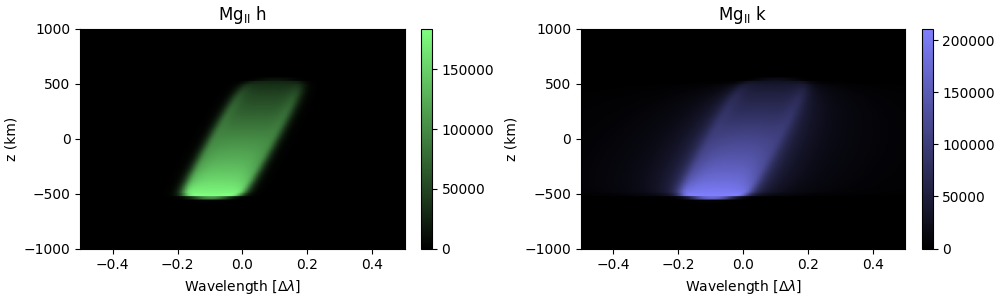
\includegraphics[width=\linewidth]{./03Modelling2D/figs/matplots/mgvrcont.png}
    \caption{The \mgiihk{} lines formed when $v_r=0.02$~rad~s$^{-1}$. The remaining parameters are the same as \fig{fig:exhmg}}
    \label{vr002c} \vspace{20pt}
    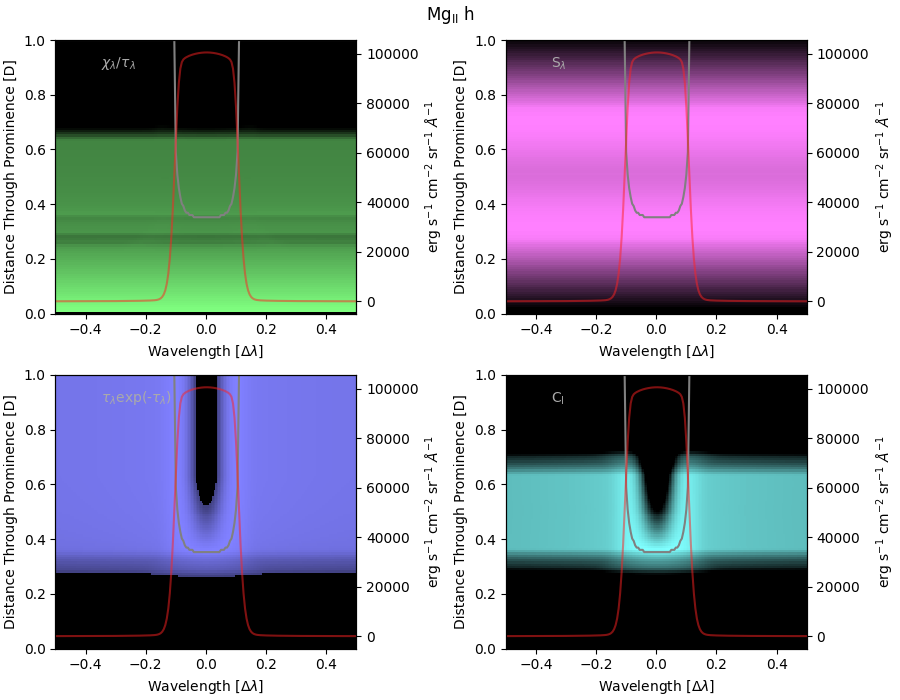
\includegraphics[width=\linewidth]{./03Modelling2D/figs/matplots/mghvr.png}
    \caption{Same as \fig{v0} but for \fig{vr002c}.}
    \label{vr002}
\end{figure}
We will now look at the simple translational velocity case where $v_y=20$\kms. All the other parameters are kept the same as in Figs. \ref{fig:exhmg} and \ref{v0}. We expect to see the same behaviour as in the static case, but with everything blueshifted. \fig{v20} shows the spectra produced by this configuration. The results are as expected, except for the discrepancies between the energy between the two cases and the shape of the line profile at $z=0$. In comparison to \fig{fig:exhmg}, we do not recover a double peak at $z=0$, but higher, we do. The non-inverted peak likely accounts for the discrepancy in energy between the static case and this $v_y\neq0$ case. \fig{vh20} appears very similar to \fig{v0} with only a Doppler shift applied.


Next we can investigate the effect of rotation on the formation of the spectra. The rotation is around the axis of rotational symmetry \seef{fig:rtcyv5}. Here the rotational velocity is set to $v_r=0.02$~rad~s$^{-1}$. This is the maximum rotation allowed by RTCY.
\begin{figure}
    \centering
    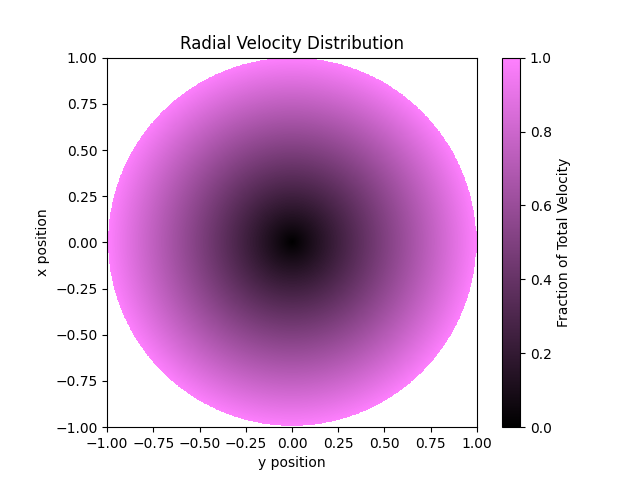
\includegraphics[width=0.45\linewidth]{./03Modelling2D/figs/vetot.png}
    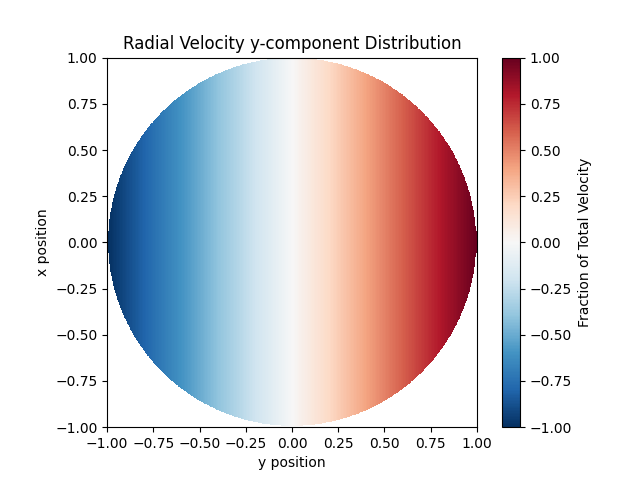
\includegraphics[width=0.45\linewidth]{./03Modelling2D/figs/vey.png}
    \caption[The velocity distribution for $v_E\neq0$ in the $xy$ plane of the simulation.]{The velocity distribution for $v_E\neq0$ in the $xy$ plane of the simulation. \textit{Left}: The total magnitude of the radial velocity at a given position. \textit{Right}: The value of $v_y$ at a given position. The observer is to the right of these plots.}
    \label{velmode}
\end{figure}

We choose this in order to see the greatest effect. The spectra produced by this can be seen in \fig{vr002c}. This result may be unsurprising as it is very similar to the $v_y\neq0$ case.  As it is rotating, the bottom of the cylinder shows the maximum blueshift, $z=0$ experiences no Doppler shift, and the top experiences the largest redshift. \fig{vr002} seems very similar to \fig{fig:exhmg}, except we also do not see a double peak here. The line profile in \fig{vr002} is formed at rest as the $vy$ component of the velocity vector is 0 at $z=0$. If we took slices of $z\neq0$, we would recover very similar plots to that seen in \fig{vh20}, with blueshift for $z<0$ and redshift for $z>0$. 

Finally, we come to the expanding case. Here, the prominence moves radially away from the axis of rotational symmetry of the cylinder, with a smooth velocity gradient such that at $D=0.5$, $v_E=0$ \seef{velmode}. As different parts of the cylinder are moving at different velocities relative to the observer, we should see interesting structure in both the spectra and the Carlsson and Stein plots. As before, all the model parameters are the same as the static case, except $v_E=20$\kms. This produces some very interesting spectra \figp{ve20c}. 
\begin{figure}
    \centering
    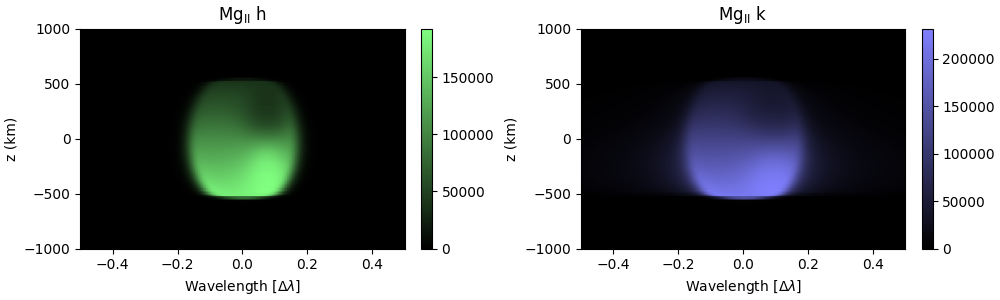
\includegraphics[width=\linewidth]{./03Modelling2D/figs/matplots/mgve20cont.png}
    \caption{The \mgiihk{} lines formed when $v_E=20$\kms. The remaining parameters are the same as \fig{fig:exhmg}}
    \label{ve20c} \vspace{20pt}
\end{figure}
\begin{figure}
    \centering
    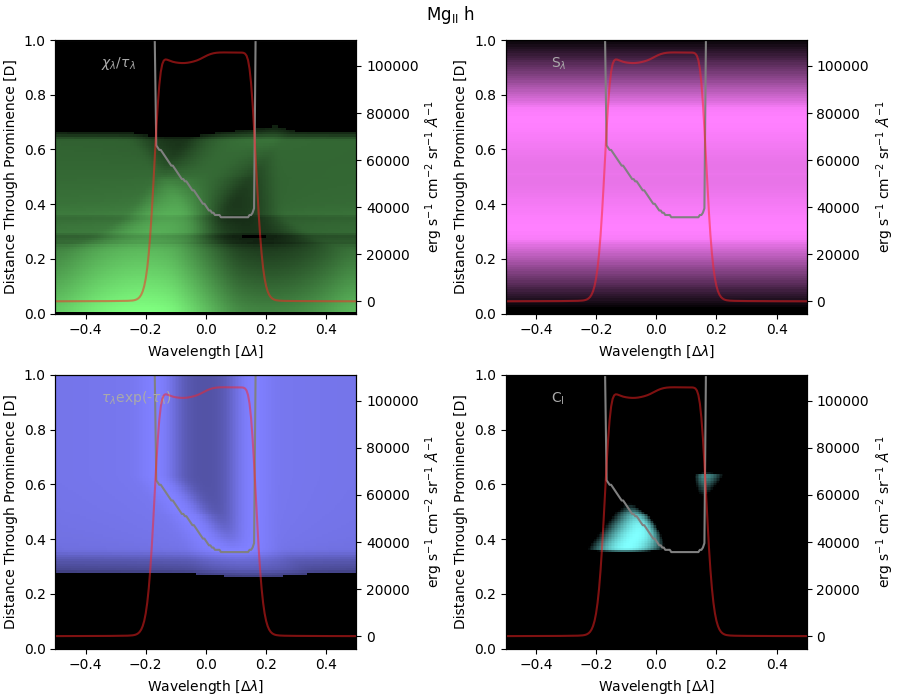
\includegraphics[width=0.9\linewidth]{./03Modelling2D/figs/matplots/mghve20.png}
    \caption{Same as \fig{v0} but for \fig{ve20c}.}
    \label{ve20}
\end{figure}
At $z=0$, all the motion is parallel to the line of sight, and as we move towards the outside edges of the cylinder, the component of velocity parallel to the line of sight changes with the cosine of the angle between the velocity vector and the line of sight. This results in a lower Doppler velocity towards the edges of the cylinder as can be seen in \fig{velmode}. This is very easily seen in the spectra as the line is broadest at $z=0$ and reduces towards the edges of the cylinder. At $z=0$, you would expect to see components of both the velocity from the front of the cylinder (antiparallel) and the back (parallel). The main effect seen here at $z=0$ is similar to Doppler dimming. The radiation from the back is not absorbed as much as in the stationary or bulk motion cases as the wavelength of the photons emitted from the back are seen to be Doppler shifted by the rest of the prominence \seef{velmode}. Therefore, radiation from the back of the prominences ($D=1$) is less absorbed as it travels through the medium towards the observer. This can be seen in \fig{ve20}, where the contribution function has a small redshifted component from the back of the cylinder. Velocity plays an important role in the spectra that we see coming from single thread prominences with the velocity distribution throughout dictating the radiation that can escape. Going forwards, we will see that it is also very important in multithread simulations.

\section{Multithread Simulations}
\begin{figure}
    \centering
    \includegraphics*[width=0.8\linewidth]{./03Modelling2D/figs/lr2016_3_new.png}
    \caption[The scenario to be considered for our first multithread test.]{The scenario to be considered for our first multithread test. This plot is based on Fig. 3 from \cite{labrosse_radiative_2016} but here we count from the back.}
    \label{lr163}
\end{figure}
RTCY allows us to simulate multithread models, albeit, not directly. We can do this by stacking the cylinders behind each other and having their radiation travel through the threads in front of them. If the cylinders are aligned, we can model this by this simple one dimensional radiative transfer equation for  two cylinders,
\begin{equation}
    I_{\lambda}=I_{\lambda,1}+I_{\lambda,0}\exp\left(-\tau_{\lambda,1}(D_1)\right).
    \label{singlert}
\end{equation}
Here we count the cylinders of the prominence from the back to the front. $I_{\lambda}$ is the outgoing specific intensity, $I_{\lambda,1}$ is the specific intensity out of the front cylinder, $I_{\lambda,0}$ is the specific intensity out of the back cylinder, and $\tau_{\lambda,1}(D_1)$ is the total specific optical depth through the front cylinder. From here on, $\lambda$ will be omitted and all radiative transfer will be assumed to be wavelength-specific. Allowing the cylinders to have various alignments, and assuming the threads do not change the internal properties of one another through irradiation, we can rewrite this equation generalised for N threads,
\begin{equation}
    I=I_N+\sum_{i=1}^{N-1}\left(I_i\exp\left(\sum_{j=i+1}^{N}-\tau_j(s)\right)\right),
    \label{totalrt}
\end{equation}
\begin{figure}
    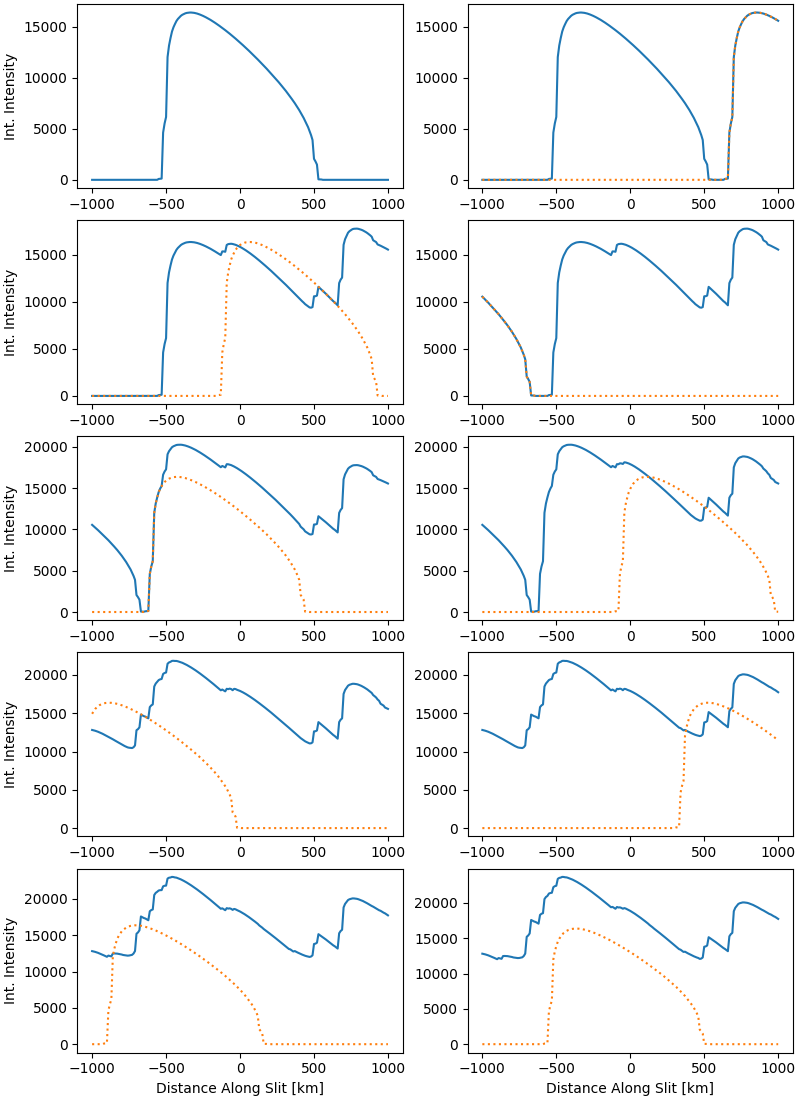
\includegraphics[width=0.49\linewidth]{./03Modelling2D/figs/Offset/MgIIh_slit.png} \hspace{1pt}\vline\hspace{1pt}
    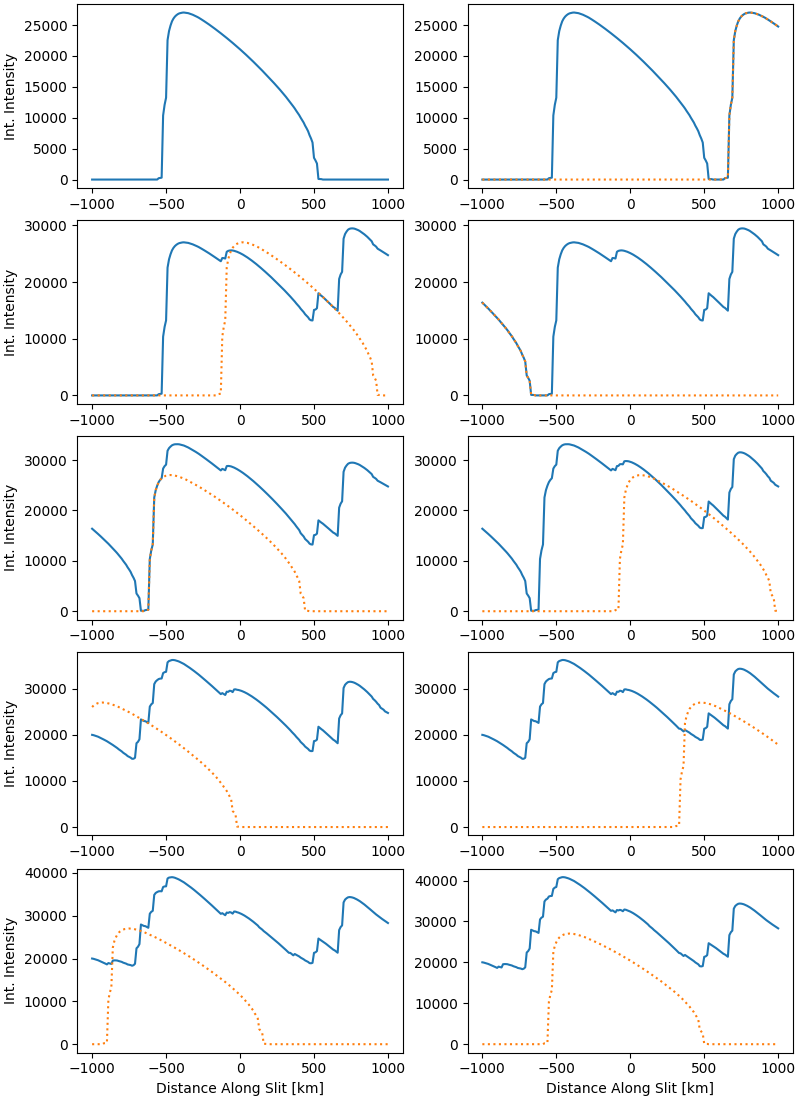
\includegraphics[width=0.49\linewidth]{./03Modelling2D/figs/Offset/MgIIk_slit.png}
    \caption[The effects of several offset structures.]{The effects of several offset structures. \textit{Left}: \mgii~h. \textit{Right}: \mgii~k. The first panel is one thread. In every subsequent panel, a new thread is added at the back. The blue line is the emergent integrated intensity, and the orange line is the integrated intensity of the newly added thread before extinction and addition. The units of the y axis are \cgsintint.}
    \label{fig:like8inlr2016}
\end{figure}

\begin{figure}
    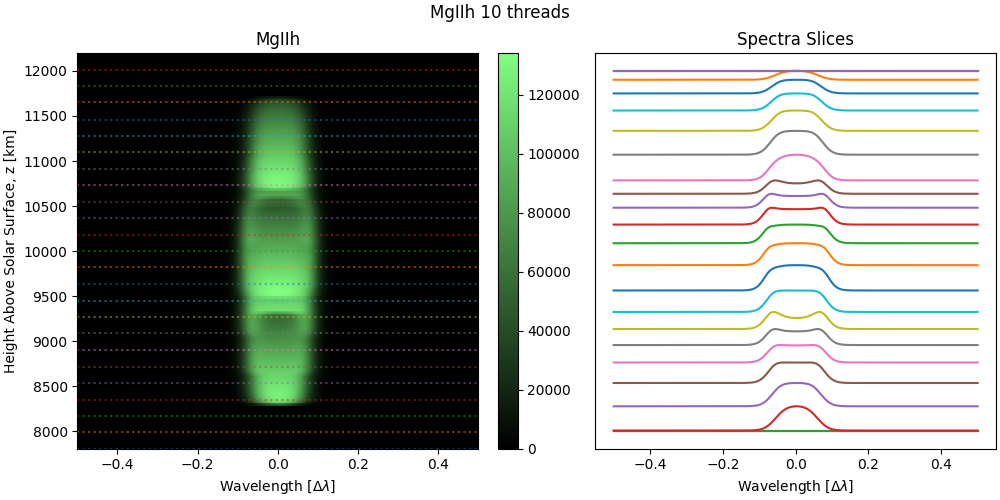
\includegraphics[width=\linewidth]{./03Modelling2D/figs/Offset/MgIIh.png}
    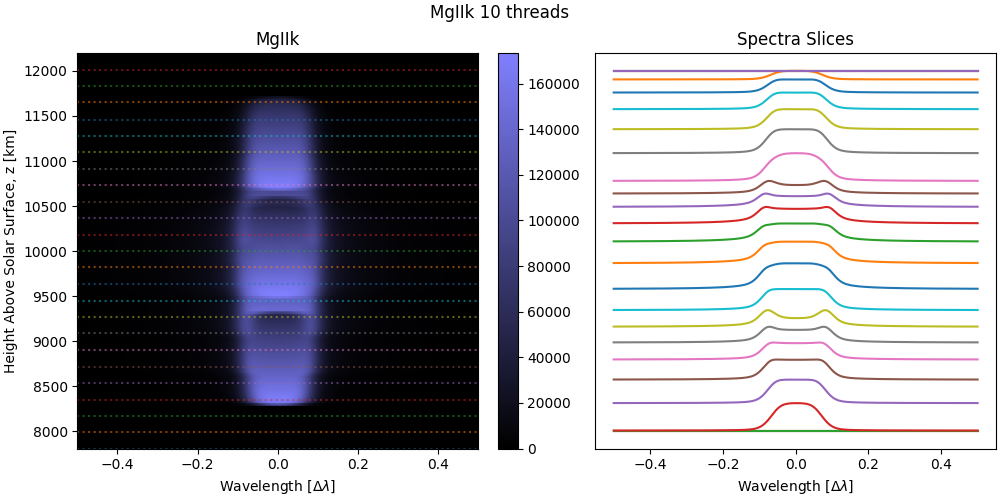
\includegraphics[width=\linewidth]{./03Modelling2D/figs/Offset/MgIIk.png}
    \caption[The emission of the stacked threads.]{The emission of the stacked threads. \textit{Top}: \mgii~h. \textit{Bottom}: \mgii~k. \textit{Left panels}: The spectroscopic view of the stacked structures. \textit{Right panels}: Slices of the spectra from the spectroscopic view. The coloured dotted lines in the left panels correspond to the same coloured line in the right panels. This plot shows the full field of view of the spectroscopic observations. \fig{fig:like8inlr2016} restricts the field of view here from 9000km to 11000km.}
    \label{fig:stackedspectra}
\end{figure}
where the first summation is over the number of threads, the second is over the number of threads proceeding $i$, $s$ is the distance travelled through cylinder $j$, and $I_N$ is the radiation from the front cylinder. Following the work done by \cite{labrosse_radiative_2016}, we first wish to investigate the effect of multiple threads on the resultant integrated \mgiihk{} intensities along the slit. Unlike \cite{labrosse_radiative_2016}, instead of starting with 10 aligned threads we begin with 10 offset threads. This set up can be seen in \fig{lr163}.
For these 10 threads, we used the same model parameters as the p4 model from \cite{labrosse_radiative_2016}; the parameters of which are $P=0.01$~dyn~cm$^{-2}$, $\alpha=\frac{\pi}{2}$, $H=10000$~km, $r_0=500$~km, $r_1=1000$~km, $T_0=6000$~K, $T_1=100000$~K, $v_T=5$~km~s$^{-1}$. These were then artificially offset to relative (to the front thread) displacements perpendicular to the line of sight of 0, -1190, -400, 1200, 90, -450, 550, -860, 370, and 30~km.

\fig{fig:like8inlr2016} shows the integrated intensity along the slit of 10 threads emitting \mgiihk{}. Unsurprisingly, these two lines produce quite similar shaped integrated intensities along the slit. \fig{fig:stackedspectra} shows the output of the spectrograph and twenty five example lines from the spectra. In this static case, it is not immediately apparent if there is more than one structure along the line of sight looking at the line profiles, however, it is more apparent looking at the integrated intensity along the slit. The number of threads remains unclear, but it is more noticeable looking at the integrated intensity along the slit.  


\begin{figure}
    \centering
    \includegraphics*[width=0.8\linewidth]{./03Modelling2D/figs/lr2016_3_vels.png}
    \caption[The scenario to be considered for our multithread test with velocities.]{The scenario to be considered for our multithread test with velocities. The redshifted threads are the negative velocities, and the blueshifted threads are the the positive velocities. This plot is based on Fig. 9 from \cite{labrosse_radiative_2016} but here we count from the back, as is convention.}
    \label{lr163v}
\end{figure}
The integrated intensity along the slit can perhaps be used as a proxy to determine if one or more structures are present in the observation. Of course, it is not clear how many there are, but it gives us more context than just the spectra. While there are a range of line profiles produced, it is not entirely obvious that several structures have created these shapes, and one would assume this emission could be from only one or two structures. This was also noted in the results of \cite{labrosse_radiative_2016} with optically thick hydrogen lines, where they also conclude that the front-most structure is most represented in the spectra produced. However, nature is rarely this organised, and it may be more pertinent to model these cylinders with random Doppler velocities. \cite{gunar_lyman-line_2008} proposed that the asymmetries seen in the Lyman lines are due to small line-of-sight velocities. To explore this effect on the \mgiihk{} lines, we will use the same velocities as used in \cite{labrosse_radiative_2016}, these velocities are 7, -7, 9, -2, -7, -9, 4, -3, 4, and -7\kms. The set up for this test is the same as in \fig{lr163} but with the above velocities applied along the line of sight \figp{lr163v}. Please note that the velocities are relative antiparallel to the LOS. Additionally, instead of running one model with the same height parameter and artificially displacing several copies to the desired height as before, here we run separate simulations for each height. We will present our plots in the same manner as Fig. 4 of \cite{gunar_lyman-line_2008}, as we feel this is the best way to show how these lines are constructed. In order to make the threads all overlap, we changed their heights to relative (to the front thread) displacements of 0~km, -119~km, -40~km, 120~km, 9~km, -45~km, 55~km, -86~km, 37~km, and 3~km, respectively.
\begin{figure}
    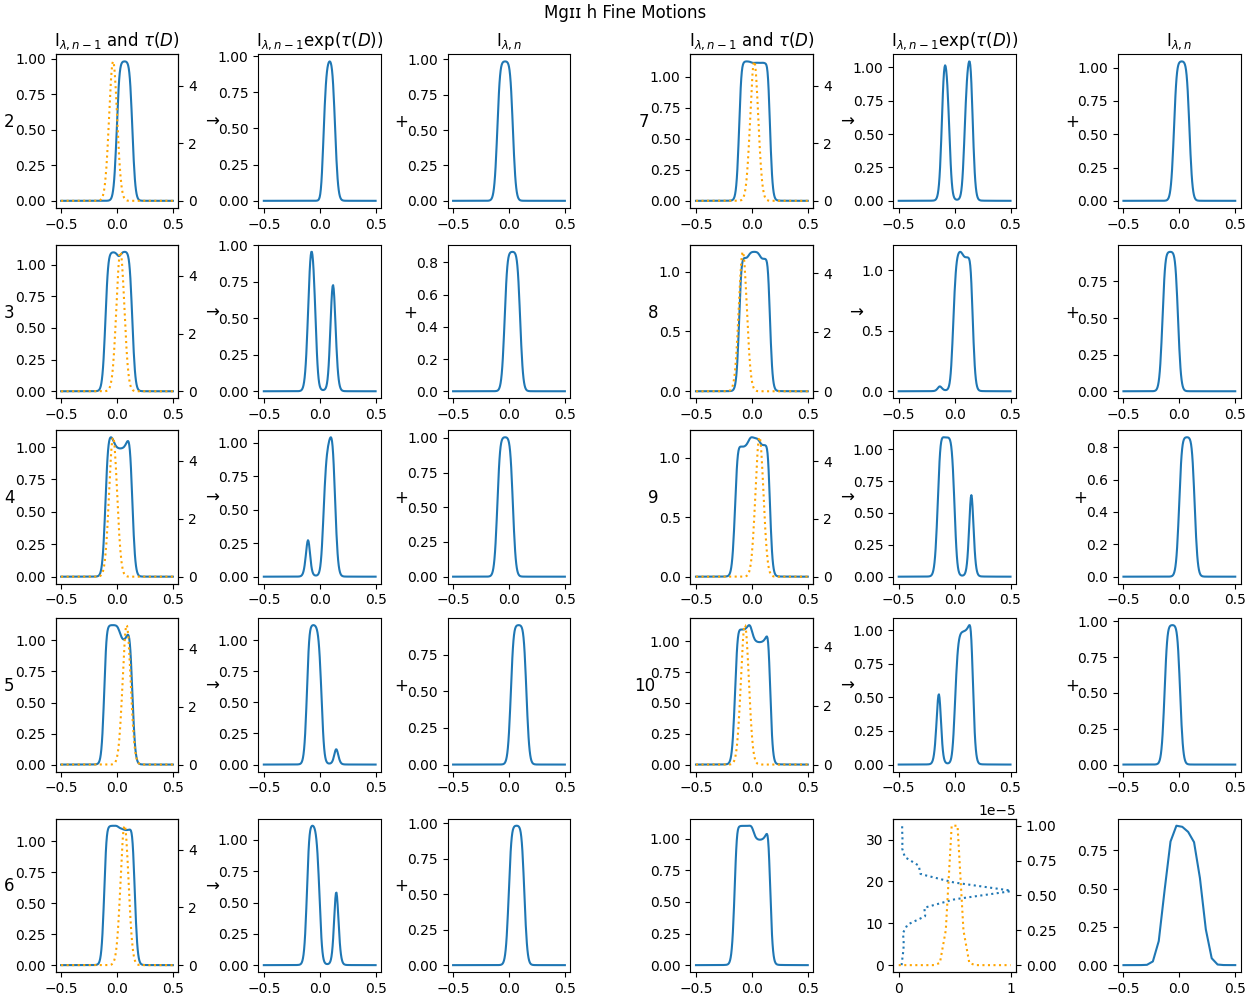
\includegraphics[width=\linewidth]{./03Modelling2D/figs/StanoPlots/slow/h.png}
    \caption[Slow Moving \mgii~h threads.]{These spectra are from the centre of the spatial window. This figure shows the step by step process of \eq{totalrt}. The number to the left of each set of three plots is $n$. Each set of the three plots are elements of the values in \eq{singlert} and are as follows: \textit{Left}: $I_{\lambda,n-1}$ in blue and $\exp\left(-\tau_{\lambda,n}(D_n)\right)$ in dotted orange; \textit{Centre}: $I_{\lambda,n-1}\exp\left(-\tau_{\lambda,n}(D_n)\right)$ in blue; \textit{Right}: $I_{\lambda,n}$. The centre and right plots are added together to create the next $I_{\lambda,n-1}$. The values of intensity are in $10^5$~\cgsint.
    The last three panels are different, and are as follows, \textit{Left}: $I_{\lambda,10}$ leaving the 10 threads. \textit{Centre}: Dotted blue: The IRIS spatial PSF where the x axis is its value normalised such that its peak is 1 and the y axis is parallel to the slit. Dotted orange: The IRIS spectral PSF where x is the normalised wavelength and y is its value normalised such that its peak is 1. \textit{Right}: The resulting line profile when convolved with the spatial and spectral PSFs of IRIS, and sampled to IRIS resolution.}
    \label{slowmgiih}
\end{figure}
\begin{figure}[h]
    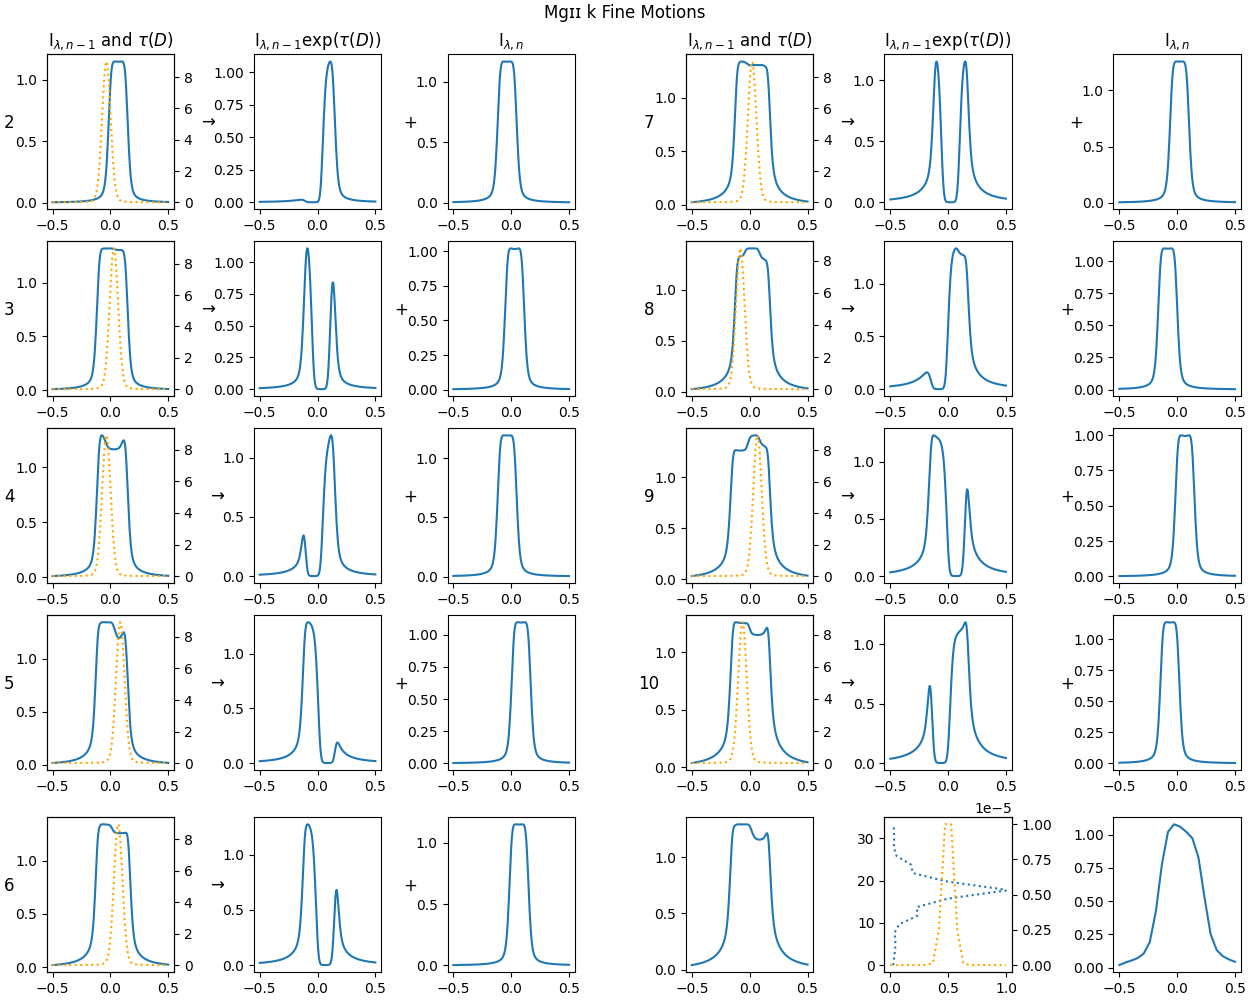
\includegraphics[width=\linewidth]{./03Modelling2D/figs/StanoPlots/slow/k.png}
    \caption[Slow Moving \mgii~k threads.]{Same as \fig{slowmgiih} but for \mgii~k.}
    \label{slowmgiik} 
\end{figure}
Additionally, similarly to  how \cite{gunar_lyman-line_2008} convolved their final line profile with the point-spread-function (PSF) of the Solar Ultraviolet Measurements of Emitted Radiation \citep[SUMER; ][]{wilhelm_sumer_1995} instrument onboard the Solar and Heliospheric Observatory \citep[SOHO; ][]{domingo_soho_1995}, we convolve our resultant line profiles with the IRIS spatial\footnote{IRIS spatial PSFs supplied by Dr Graham S. Kerr.} and spectral PSFs. The spectral PSF takes the form of a Gaussian with a full width half maximum (FWHM) of 2 pixels \citep{depontieu_interface_2014}. This translates to a FWHM of approximately 0.1~\AA{} for the NUV filter. This may seem negligible, but it has a striking effect when combined with the spatial PSF. In order to formulate this Gaussian, we must convert from FWHM to the standard deviation. To do this we use the following relationship \citep{weisstein_gaussian_2022},
\begin{equation}
    \sigma=\frac{f}{2\sqrt{2\ln(2)}},
\end{equation}
where $f$ is the FWHM, and $\sigma$ is the standard deviation of the Gaussian. Substituting 0.1~\AA{} in for $f$, we get a standard deviation of approximately 0.042~\AA.

The spatial PSF assumes a resolution of 0.166\arcsec{} along the spatial axis of the spectrograph. At 1~AU this is 120.88~km. The resolution of our simulations is 10~km, or 0.0134\arcsec{} at 1AU. Therefore the spatial PSF is resampled and normalised to fit the resolution of our simulations. In practice, this should also be done when deconvolving IRIS observations, but is currently ignored by the official deconvolution routine.
\fig{slowmgiih} and \fig{slowmgiik} show the results of these 10 stacked threads convolved with the IRIS spatial and spectral PSFs. 
These plots show the spectra from the centre of the spatial window and the step by step process of \eq{totalrt}. The number to the left of each set of three plots is $n$. These sets of three plots correspond to elements of the values in \eq{singlert}. The last three panels are different; they show the resulting line profile when it is convolved with the spatial and spectral PSFs of IRIS, and sampled to the resolution of IRIS.
The final line profiles are only slightly asymmetrical. If these were seen in an IRIS observation, they would be assumed to be a single profile from a single thread. However, they are not. The only clue towards their true nature is the large FWHM created by the relatively lower optical thickness in the wings of \mgiihk.
This may lead to an incorrect assignment of a large microturbulent velocity. This is not entirely unreasonable however, as this can account for the now unresolved fine motions present. Usually, microturbulent velocities are unresolved stochastic motions in the plasma, but they can used as a proxy for unresolved fine motions like this as they widens the line profile in a similar way.

Although \mgiihk{} are optically thick like Ly~$\beta$, we do not recover as striking an asymmetry as \cite{gunar_lyman-line_2008} with Ly~$\beta$. However, the standard shape of a Ly~$\beta$ line profile lends itself to be heavily affected as its double peaks are separated by almost 0.5~\AA. The double peaks of \mgiihk{} are not as far apart, and the majority of line profiles from these threads are single peaked. To produce more pronounced asymmetries in \mgiihk{}, faster moving threads would required. 
\begin{figure}
    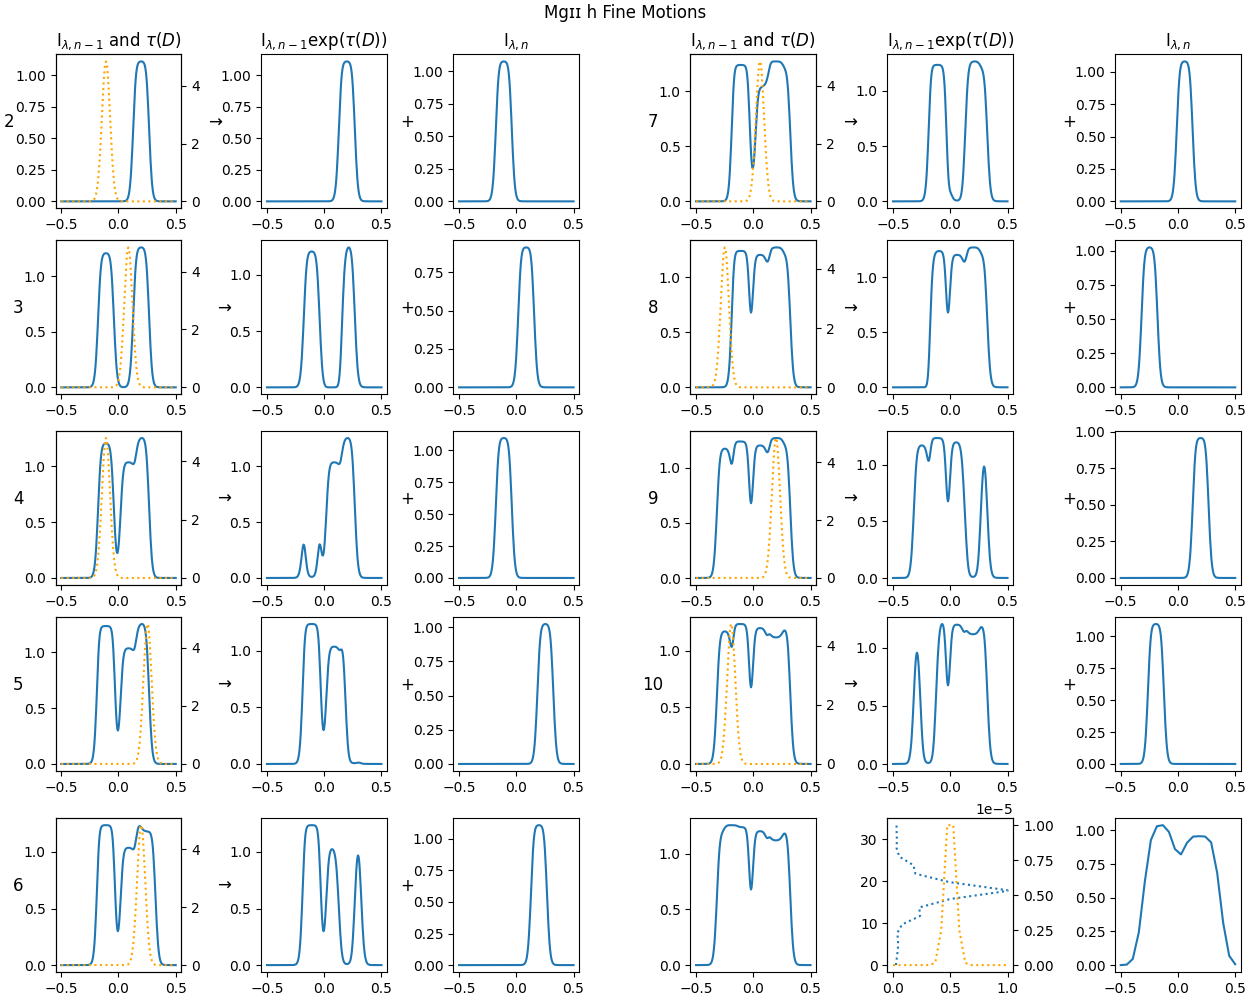
\includegraphics[width=\linewidth]{./03Modelling2D/figs/StanoPlots/fast/h.png}
    \caption[Fast Moving \mgii~h threads.]{Same as \fig{slowmgiih} but for fast moving \mgii~h.}
    \label{fastmgiih}
\end{figure}
This simulation was repeated with all of the velocities were by three, resulting in 21\kms, -21\kms, 27\kms, -6\kms, -21\kms, -27\kms, 12\kms, -9\kms, 12\kms, and -21\kms. 
These higher velocities are still of reasonable magnitude, as in \sect{velsect} and \sect{rrms} we showed that the range of velocities observed in our prominence were mainly in the range -25\kms{} to 25\kms{}. This is consistent with that reported in the review by \cite{labrosse_physics_2010}. \fig{fastmgiih} and \fig{fastmgiik} show the results from these faster moving threads. The final line profile (before convolution) in \fig{fastmgiih} is very interesting, it is unfortunate that the PSF of IRIS destroys these features. However, we do recover asymmetry. It manifests itself as standard asymmetric double peaked profile.  The same can be said about the final profile in \fig{fastmgiik}, but there is still some complex structure present in the profile. The difference between \mgiihk{} is due to the larger line width of \mgii~k. 
\begin{figure}
    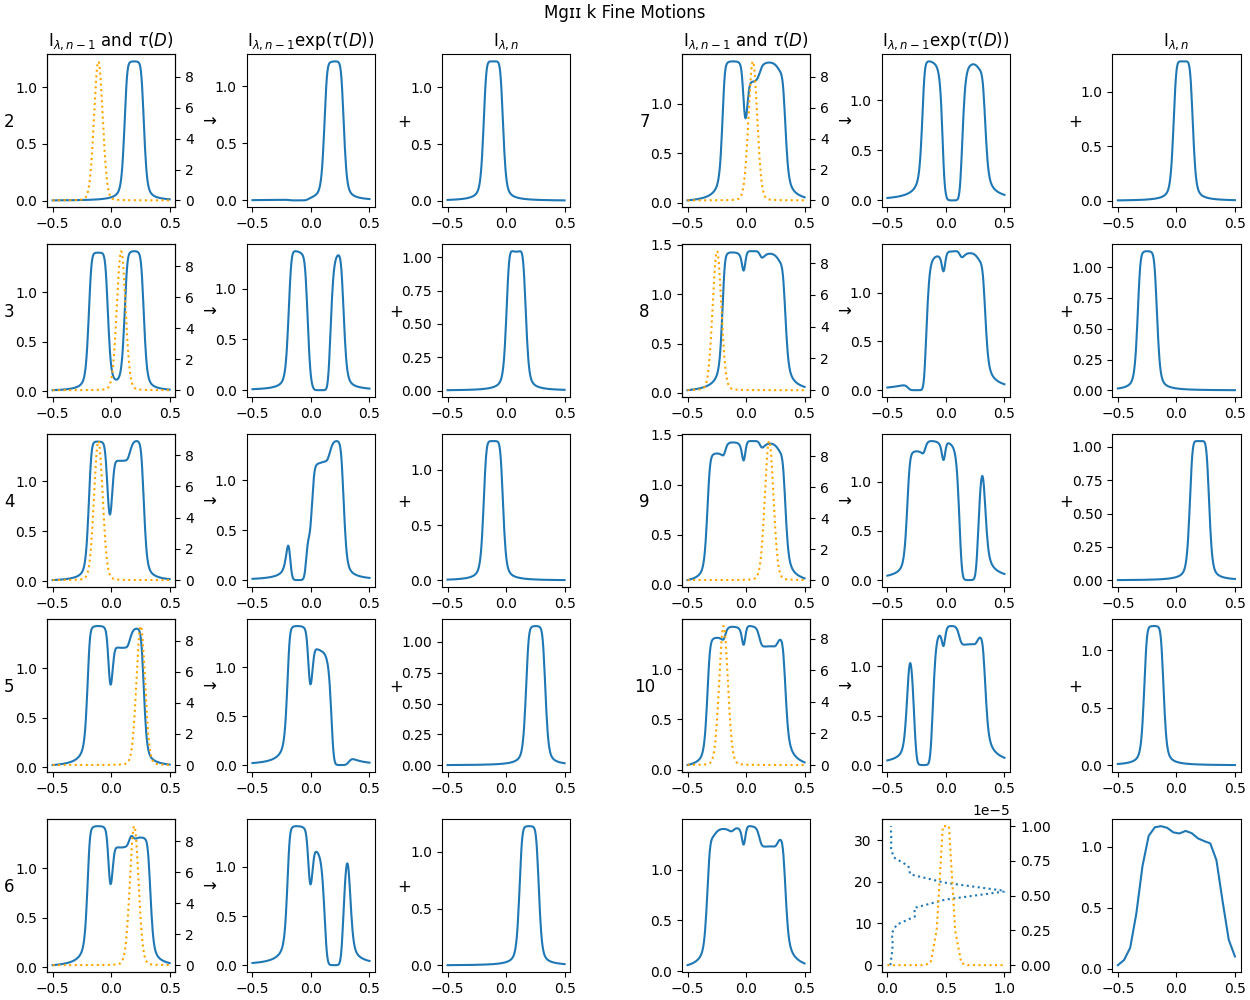
\includegraphics[width=\linewidth]{./03Modelling2D/figs/StanoPlots/fast/k.png}
    \caption[Fast Moving \mgii~k threads.]{Same as \fig{fastmgiih} but for \mgii~k.}
    \label{fastmgiik}
\end{figure}
Much more of the 1~\AA{} window can be filled by \mgii~k. This is very apparent in the last set of three panels of \fig{fastmgiik}, where the line profile just fits within the window. As IRIS observations, these could be interpreted as three to four structures, and not ten. Following the comments from the previous zero velocity thread test, we said that the front-most thread was most represented in the spectra. From this it may be concluded that using ten threads is excessive. However, we can investigate this by simply looking at the contribution of the back-most thread to the final line profile. Modifying \eq{totalrt}, to remove the emission from the other threads, we can look at only how emission from the the back-most thread is absorbed,
\begin{equation}
    I_C=I_0\exp\left(\sum_{j=1}^N-\tau_j(s)\right),
\end{equation}
where $I_C$ is the contributed intensity, $I_0$ is the outgoing intensity of the back-most thread, and $\tau_j$ is the optical thickness of the threads in front of the back-most thread.
\begin{figure}
    \centering
    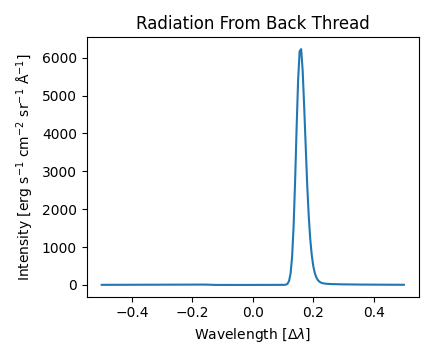
\includegraphics[width=0.49\linewidth]{03Modelling2D/figs/slowback.png}
    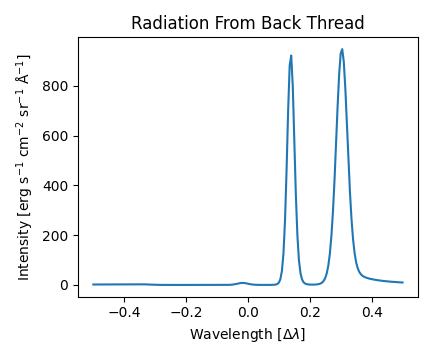
\includegraphics[width=0.49\linewidth]{03Modelling2D/figs/fastback.png}
    \caption[The contribution of the back-most thread to the final profile.]{The contribution of the backmost thread to the final profile for \mgii~h. \textit{Left}: The slow-moving case. \textit{Right}: The fast-moving case.}
    \label{backthreads}
\end{figure}
\fig{backthreads} shows the radiation from the back-most thread that escapes from the front of thread 10. Surprisingly, the faster moving threads are more heavily absorbed than their slow counterparts. This is likely due to a large optical thickness lining up with the peak in the spectrum from the fast moving back-most thread. Threads 5, 6, and 9 appear to be the culprits. Their optical thicknesses all align with the line core of thread 1 \seef{fastmgiik}. This does not happen in the slow-moving case. The optical thicknesses of the other threads do not line up exactly with the line core. Half of the line profile is missing, however, but it has not lost as much of its peak.
Overall, the back-most thread accounts for 0.6\% of the total outgoing radiation for the slow-moving configuration, meanwhile the back-most thread contributes 0.009\% of the total outgoing radiation for the fast-moving configuration. This is almost negligible, therefore fewer threads may have been sufficient. 
\begin{figure}
    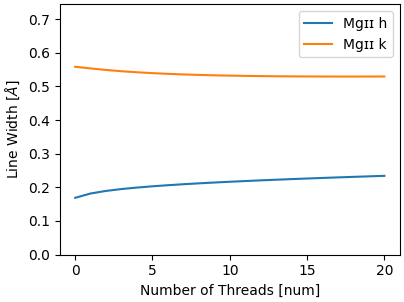
\includegraphics[width=0.49\linewidth]{./03Modelling2D/figs/stak.png}
    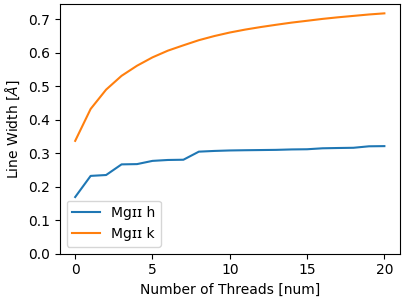
\includegraphics[width=0.49\linewidth]{./03Modelling2D/figs/stac.png}
    \caption[The effect that multiple aligned stacked threads have on the line width.]{The effect that multiple aligned stacked threads have on the line width. \textit{Left}: The static case. \textit{Right}: The moving case.}
    \label{lwzoom}
\end{figure}

Another test we can do to investigate how many threads are sufficient in such a configuration is to investigate how line width changes with the number of threads. Here, we define line width as in \eq{eq:fwhm} using the quantile method and for the threads we use the p4 model from \cite{labrosse_radiative_2016}. \fig{lwzoom} shows the result of this stacking. On the left we have all aligned stationary threads, and on the right, the threads are all aligned with random LOS velocities in the range $-$10\kms{} to 10\kms. In the static case, it is very obvious that the line width does not change much with the number of threads. The initial drop in line width for \mgii~k is due to more and more of the intensity focusing near the centre. This is not seen in \mgii~h as this is an effect of the CRD treatment of these lines which causes \mgii~k to have a very large line width. After approximately 10 threads, they begin to converge. As for the threads with random LOS velocities, the behaviour is different. \mgii~h appears to have converged after 9 threads, but \mgii~h continues to rise. Logically, you would expect these to converge towards the same value, which is the width of wavelength range over which the the LOS velocities can shift the lines to. So, in the case of high velocities, due to the effect on the line width, 10 may not have been enough for \mgii~k to demonstrate this effect to its fullest. For static threads, however, 10 does indeed seem sufficient.

These multithreaded simulations have shown that even small asymmetries noticed by IRIS may be the result of many threads along the line of sight moving at different velocities. Unfortunately, it has also highlighted how the PSFs of IRIS cause us to lose crucial detail in these profiles and therefore may cause us to draw incorrect conclusions about the properties of the emitting plasma. 

\section{Multithread Forward Fit}
\label{2dinvert}

\begin{figure}
    \centering
    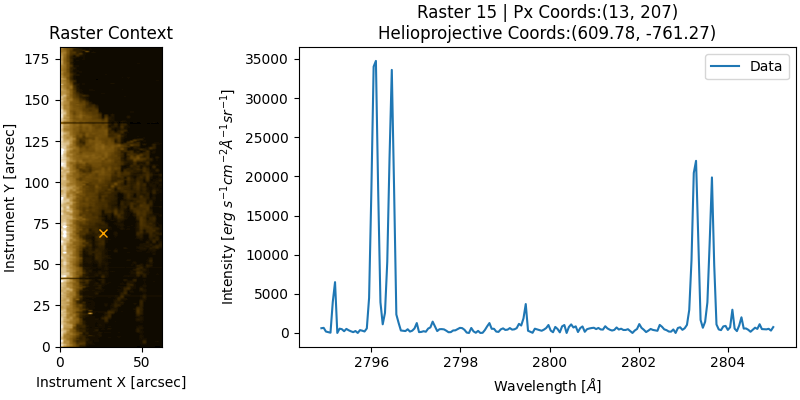
\includegraphics[width=\linewidth]{./03Modelling2D/figs/invert/spectratoimvert.png}
    \caption{An example spectrum that we wish to attempt to invert with multithread models.}
    \label{spec2inv}
\end{figure}
As promised in \sect{xrms}, to conclude this chapter, we will manually invert the spectra in \fig{spec2inv} with a multithread model. We will do this by forward fitting. Henceforth, we will refer to the largest set of peaks as the first thread, and the second set of peaks as the second thread. Luckily, we have an initial guess for the first thread from xRMS. 
\begin{figure}[h]
    \centering
    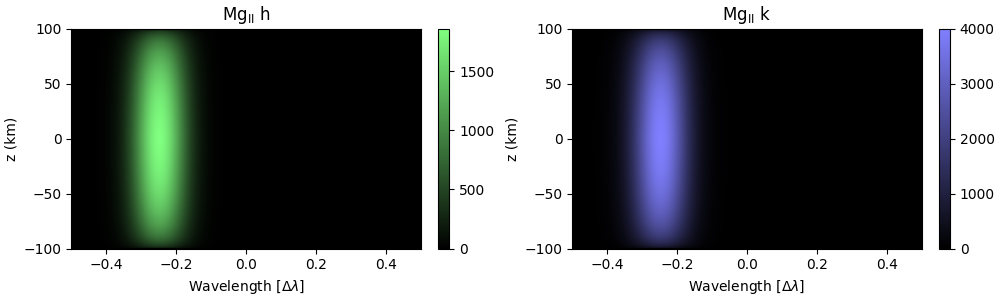
\includegraphics[width=\linewidth]{./03Modelling2D/figs/invert/test1.png}
    \caption[The \mgiihk{} spectra generated by RTCY with the parameters found by xRMS.]{The \mgiihk{} spectra generated by RTCY with the parameters found by xRMS. The colour bar units are \cgsint. The parameters of this simulation are $T=8000$~K, $P=0.02$\dyncm, $D=200$~km, $v_T=8$\kms, $H=10000$~km, $v_y=-27$\kms{}, and $v_z=80$\kms.}
    \label{prom2d} \vspace{20pt}
    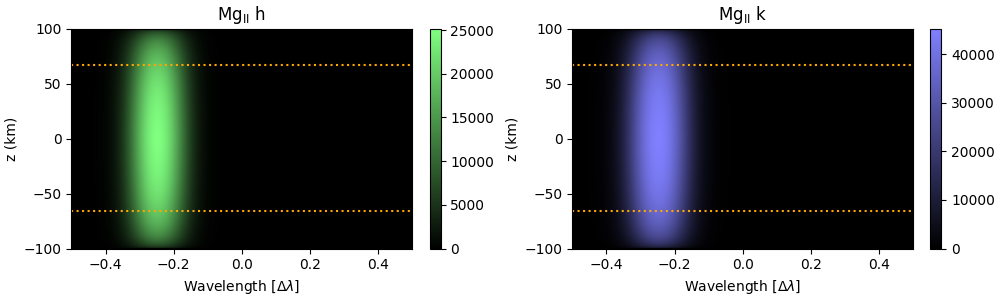
\includegraphics[width=\linewidth]{./03Modelling2D/figs/invert/good.png}
    \caption[The \mgiihk{} spectra generated by RTCY with $T=7000$~K.]{The \mgiihk{} spectra generated by RTCY with $T=7000$~K. The dashes orange lines are the position which the 1D spectra are taken from. The colour bar units are \cgsint. The parameters of this simulation are $T=7000$~K, $P=0.02$\dyncm, $D=200$~km, $v_T=8$\kms, $H=10000$~km, $v_y=-27$\kms{}, and $v_z=80$\kms.}
    \label{prom7k}
\end{figure}
These are the following parameters, $T=8000$~K, $P=0.02$\dyncm, $D=200$~km, $v_T=8$\kms, $H=10000$~km, a Doppler velocity along the line of sight of $-27$\kms, and an outwards radial velocity of 80\kms.  
This is an isothermal model as $\gamma=0$ at that particular pixel. We set $\alpha=0$ so that we may check individual slices of the spectra while making sure that $D=200$~km along the slit. If $\alpha\neq0$ then $D$ would change along the slit as the slit is no longer aligned with the axis of rotational symmetry. \fig{prom2d} shows the result from this simulation. Unfortunately, they do not reach the required intensity  to be indicative of plasma properties at this pixel. They only reach approximately 10\% of the required intensity. However, by dropping the temperature to 7000~K, we recover high enough intensities \figp{prom7k}. After manually searching through slices of the 1D spectra, two ranges of candidate $z$-slices were selected in both \mgii~h and \mgii~k. This was done by checking the peak intensity of the slices against that of the peaks of the first thread in the data. These ranges in $z$ are areas where the 1D spectra reach a high enough intensity to be comparable with that of the data. However, these ranges in h and k did not overlap. Instead then, the $z$ slice between each of the pairs of ranges were selected as the candidate slices. These two new candidates were both within 4~km of the candidate ranges. The two candidate slices are located at -66~km and 67~km relative to 10000~km in $z$. These two slices are chosen from the top and bottom of the prominence as the incident radiation received will be different. \fig{prom7k} shows the location of these two slices as dotted orange lines. \fig{models} shows the 1D spectra of these two slices padded with zeros so that they may be compared. For the second thread that xRMS did not match, we assume that it is of the same properties as the first thread and is behind it.
\begin{figure}
    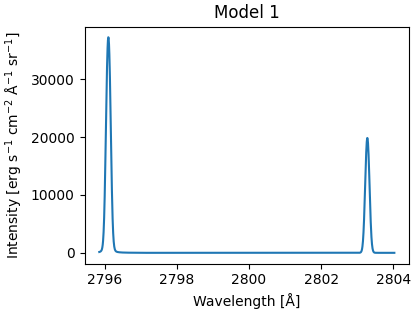
\includegraphics[width=0.49\linewidth]{./03Modelling2D/figs/invert/model1.png}
    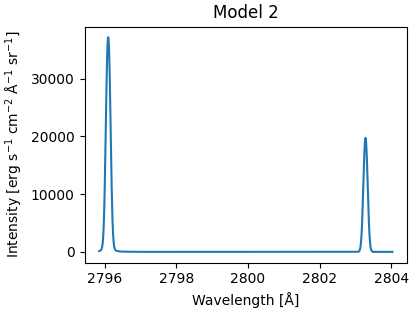
\includegraphics[width=0.49\linewidth]{./03Modelling2D/figs/invert/model2.png}
    \caption[The model candidates for the considered spectra.]{The model candidates for the considered spectra. \textit{Left}: The model from the -66~km slice. \textit{Right}: The model from the 67~km slice.}
    \label{models} \vspace{20pt}
    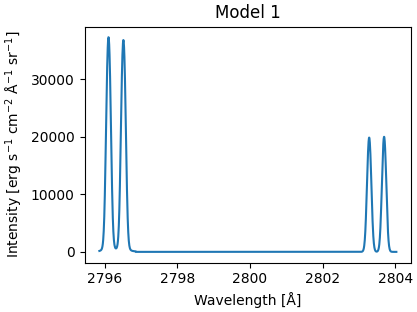
\includegraphics[width=0.49\linewidth]{./03Modelling2D/figs/invert/model1tot.png}
    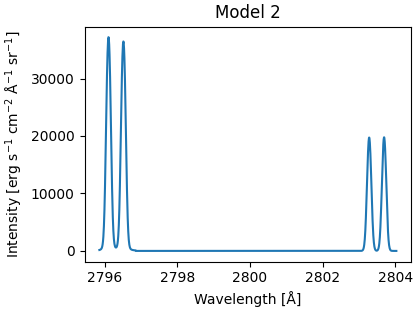
\includegraphics[width=0.49\linewidth]{./03Modelling2D/figs/invert/model2tot.png}
    \caption[The combined model candidates for the considered spectra.]{The combined model candidates for the considered spectra. \textit{Left}: The models from the -66~km slice. \textit{Right}: The models from the 67~km slice.}
    \label{modelsfull}
\end{figure}
\begin{figure}
    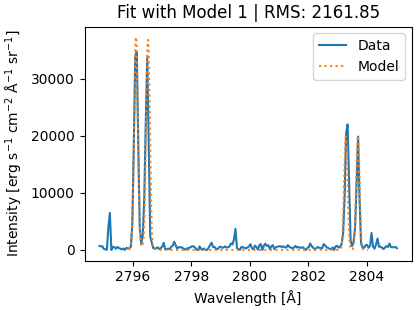
\includegraphics[width=0.49\linewidth]{./03Modelling2D/figs/invert/invert1.png}
    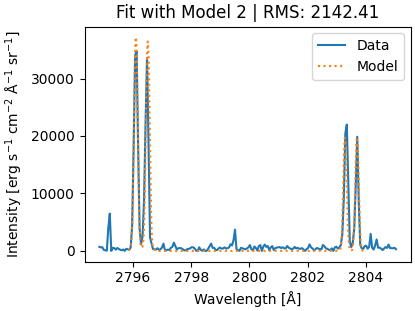
\includegraphics[width=0.49\linewidth]{./03Modelling2D/figs/invert/invert2.png}
    \caption[The model matches and their associated RMS.]{The model matches and their associated RMS. \textit{Left}: The models from the -66\kms{} slice. \textit{Right}: The models from the 67\kms{} slice.}
    \label{lastmodelfit}
\end{figure}
Its lower intensity being a result of it transmission through the first thread. We need to measure the Doppler velocity of the peaks of the second thread in order to create a model with that Doppler velocity. The quantile method cannot be used here, as the peaks from both threads are too close together. Instead, the peaks were measured manually. The peak wavelength of the \mgiihk{} peaks of this thread were determined to be 2769.50~\AA{} and 2803.70~\AA{}. Then using the following form of the Doppler equation to calculate their Doppler velocity,
\begin{equation}
    v=\frac{c(\lambda-\lambda_0)}{\lambda_0},
\end{equation}
where $v$ is the Doppler velocity, $\lambda_0$ is the rest wavelength of the line, $\lambda$ is the observed wavelength, and $c$ is the speed of light ($3\times10^5$\kms), their Doppler velocities were found to be 17.17\kms{} and 17.12\kms{}, respectively. The mean of these velocities, 17.145\kms{} was then used to generate a second model with the same parameters as the first thread, except with this 17.145\kms{} as the Doppler velocity. The two models were then added together, taking care to account for the optical thickness of the first. The result of the addition of these models can be seen in \fig{modelsfull}. Now we can calculate the best fitting of these two models through RMS. 

The RMS of Model 1 was 2161.85, and Model 2 was 2142.41 \seef{lastmodelfit}. These are well below the 15000 threshold set for xRMS on this prominence. Even though marginally, model 2 is the best fitting. This means that the height of the prominence is approximately 10066~km with the following other parameters, $T=7000$~K, $P=0.02$\dyncm, $D=200$~km, and $v_T=8$\kms. The only disagreement between this multithread forward fit and xRMS is the temperature of the model. xRMS found this to be 8000~K, and this forward fit found it to be 7000~K. A more accurate value may be somewhere between these two temperatures.

\section{Concluding Remarks}
2D modelling is a very powerful tool for understanding the formation of line profiles. We see that in the case of an expanding cylinder, due to the range of velocities throughout the cylinder, material from the back, which would be absorbed in the static case, is able to transmit, creating asymmetry that may be seen in observation. Stacking many unaligned static threads however fails to produce complex spectra due to the optical thickness of the lines. This effect is not as pronounced as it was in \cite{labrosse_radiative_2016} with Ly$\alpha$, as the wings of the \mgiihk{} lines experience some enhancement. When different velocities are introduced however, complex line profiles do arise -- even with velocities in the range 0 to 10\kms, similar to what was found by \cite{gunar_lyman-line_2008} for Ly$\beta$ and \cite{labrosse_radiative_2016} for H and He lines. By increasing the velocities to three times their original value, such that they are in the range 0 to 30\kms{}, we recover yet more complex line profiles. However, through the convolution with the IRIS spatial and spectral point-spread-functions, these complex structures are smoothed out and take on the appearance of a more classical \mgiihk{} double peak. Using 2D modelling to invert prominence spectra as done in Chap. \ref{Chap:prom}, is not trivial. Every spectrum has 201 spectral slices, so a manual forward fit was done on one pixel as a proof of concept. We were able to recover a satisfactory multithread solution for this pixel well below the RMS limit set for rRMS and xRMS in Sects. \ref{rrms} and \ref{xrms}.